\section{Implementation}
\subsection{Overview}
The project will solve PdM hurdles for operators in modernized workplaces by providing an accurate estimate of asset health.
The proposed method is to replicate the results achieved by other papers using SOMs for condition monitoring. 
Specifically, to train a SOM and get a health score by calculating how much a test data point deviates from normal operation.
The higher the health score, the lower the operating condition of the asset.
%Various SOM implementations will be examined, such as the \href{https://pypi.org/project/kohonen/}{Kohonen 1.1.2 Python package} (documentation for this package is sparse).
%If these do not provide enough customization then a SOM will be self-coded using Tensorflow.
%Customization may be required to allow the comparison of various distance metrics to get a health score.
As discussed, this has been done before but is rarely seen in industry today and the use of these algorithms on real and significant data is challenging and relevant.
For example, the data will be provided in hourly chunks throughout the year (instead of one continuous data set).
Furthermore, feature engineering techniques are be explored to improve performance, use-ability and interpretability.
%Decision boundaries will be learned as a final step (if we have enough failure data) to organize failures into different classes and severity levels.
\begin{figure}[!h]
    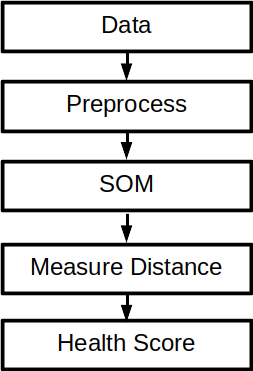
\includegraphics[width=3cm]{steps}
    \centering
    \label{fig:steps}
    \caption{Implementation steps from Data.}
\end{figure}

\subsection{Feature Engineering}
There are vibration signals used for the following: the interior bearing of the fan, 
the outer bearing of the fan, 
the interior bearing of the motor, and
the outer bearing of the motor (Figure \ref{fig:raw-signals}). 
The mean, standard deviation, skewness, kurtosis, and peak to peak were calculated every five minutes for each of the variables.
These five time domain features are commonly used to describe a signal \cite{Tian2014AnomalyDU}.
Additionally, the correlation between the signal and the other three was added as it increased the performance of the SOM.

\begin{figure}[!h]
    \centering
    \begin{subfigure}{6cm}
        \centering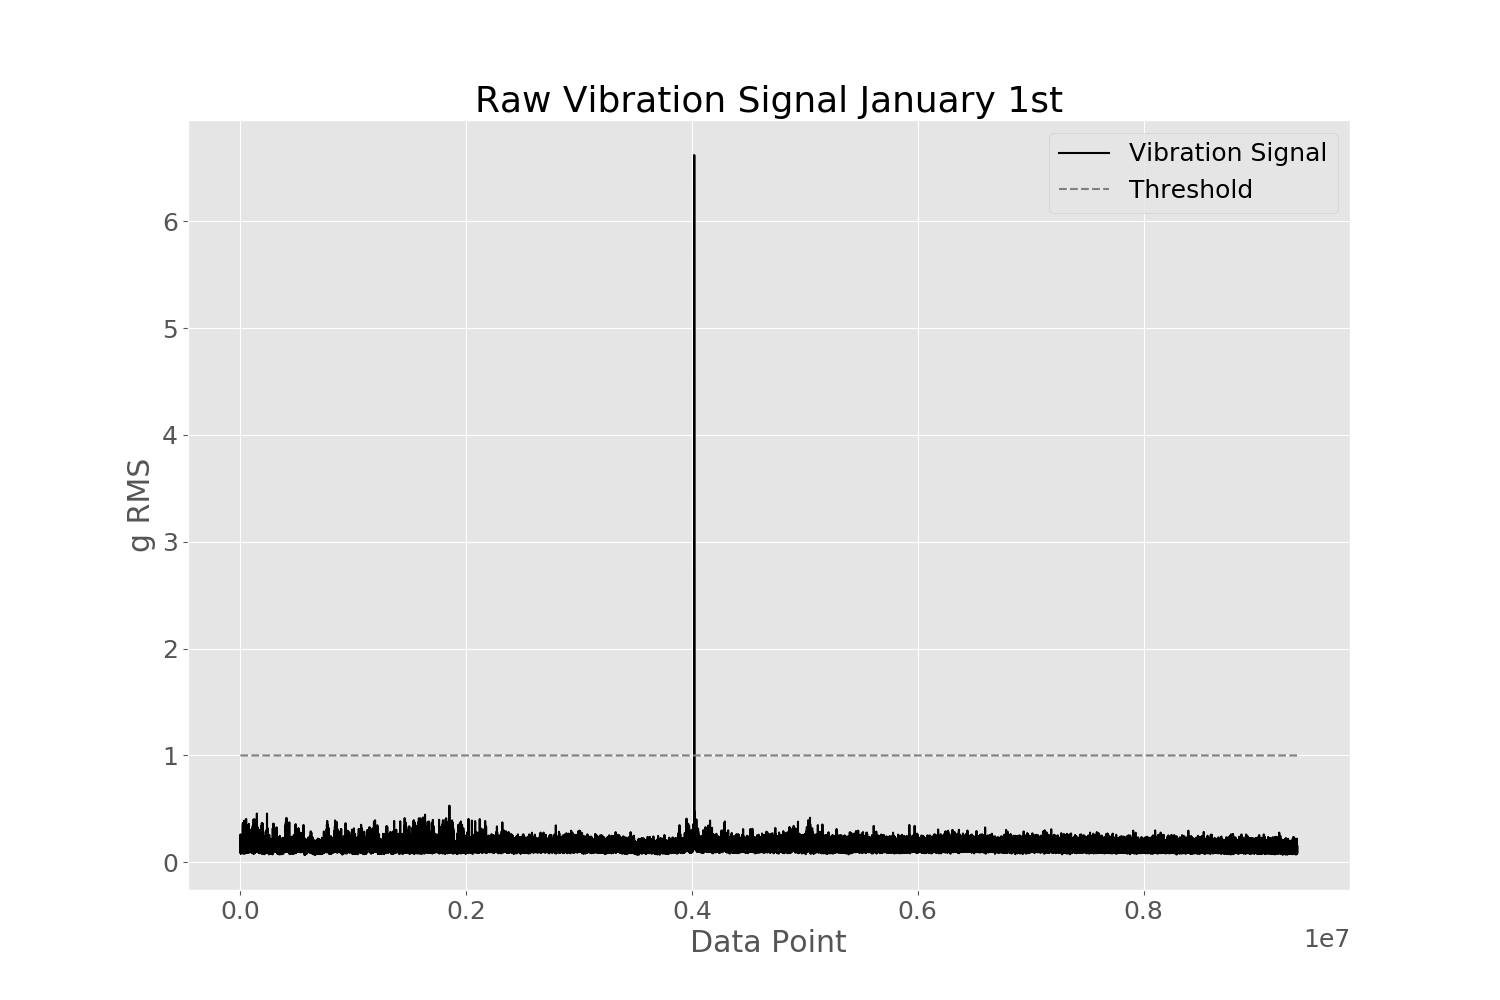
\includegraphics[trim={300 50 50 50}, width=\linewidth]{raw-jan1}
    \end{subfigure}%
    \begin{subfigure}{6cm}
        \centering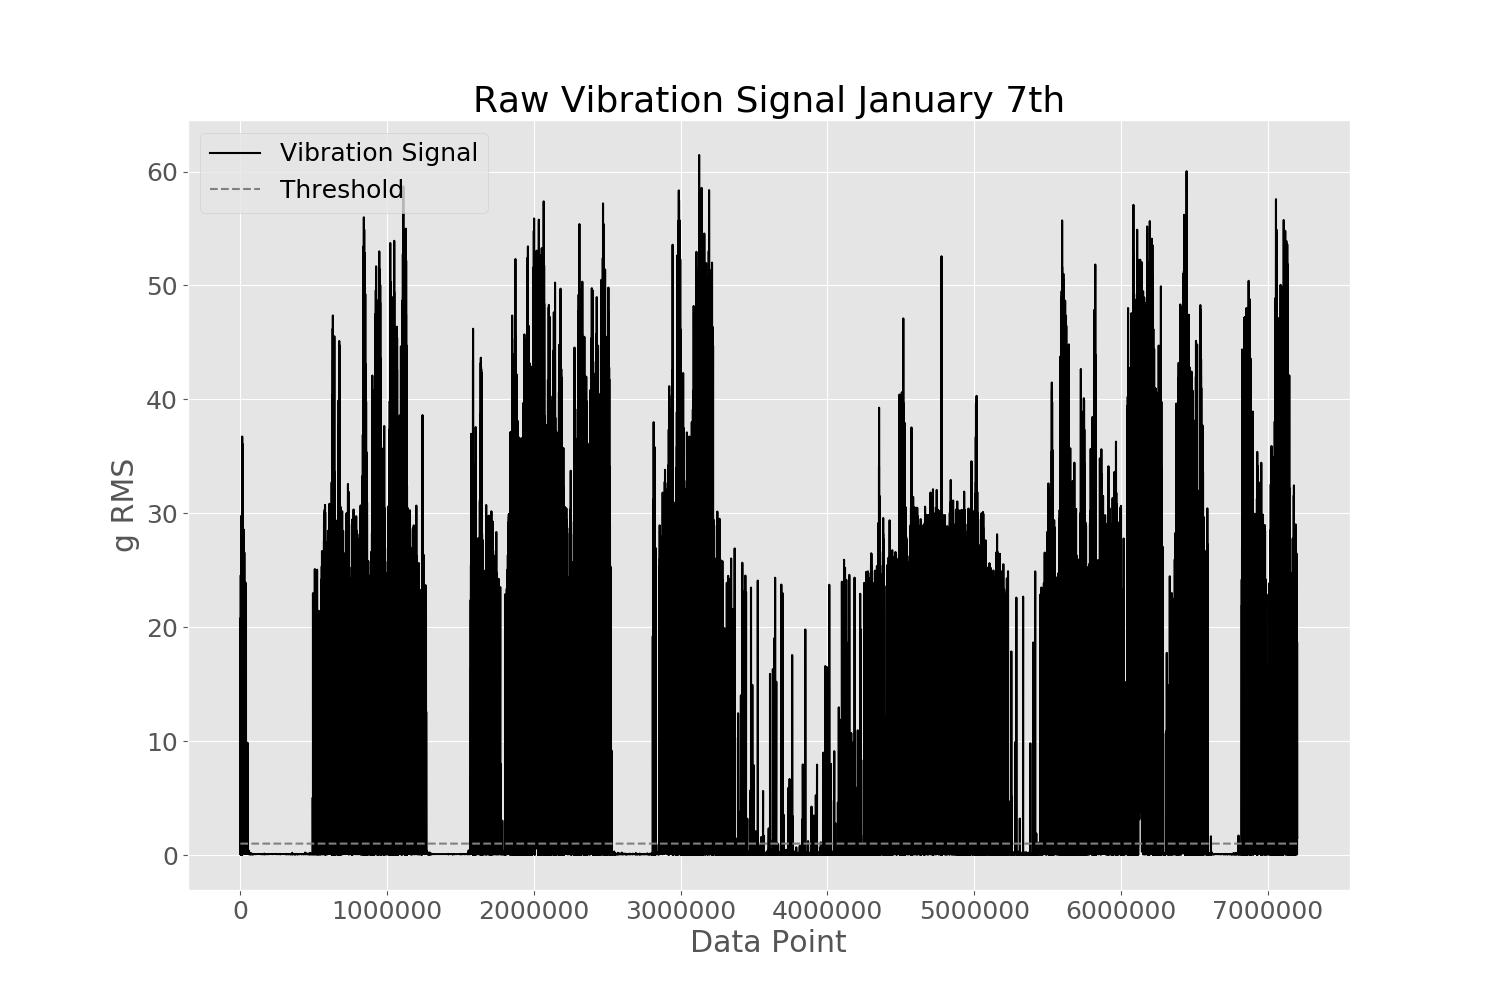
\includegraphics[trim={50 50 300 50}, width=\linewidth]{raw-jan7}
    \end{subfigure}\vspace{10pt}
 
    \begin{subfigure}{6cm}
        \centering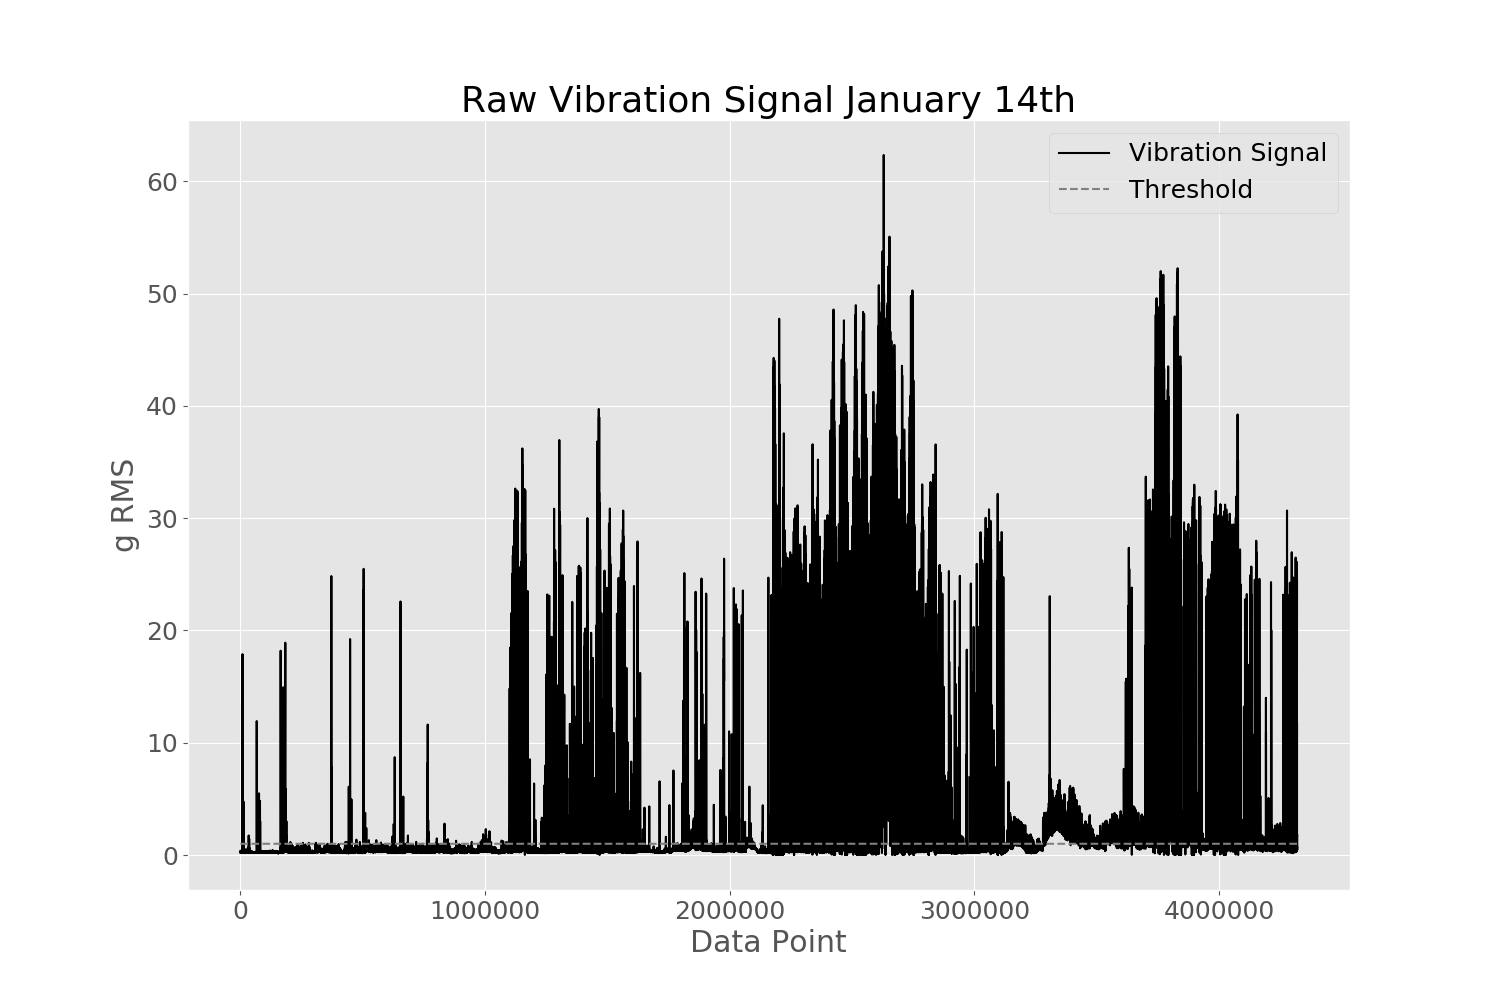
\includegraphics[trim={300 50 50 50}, width=\linewidth]{raw-jan14}
    \end{subfigure}%
    \begin{subfigure}{6cm}
        \centering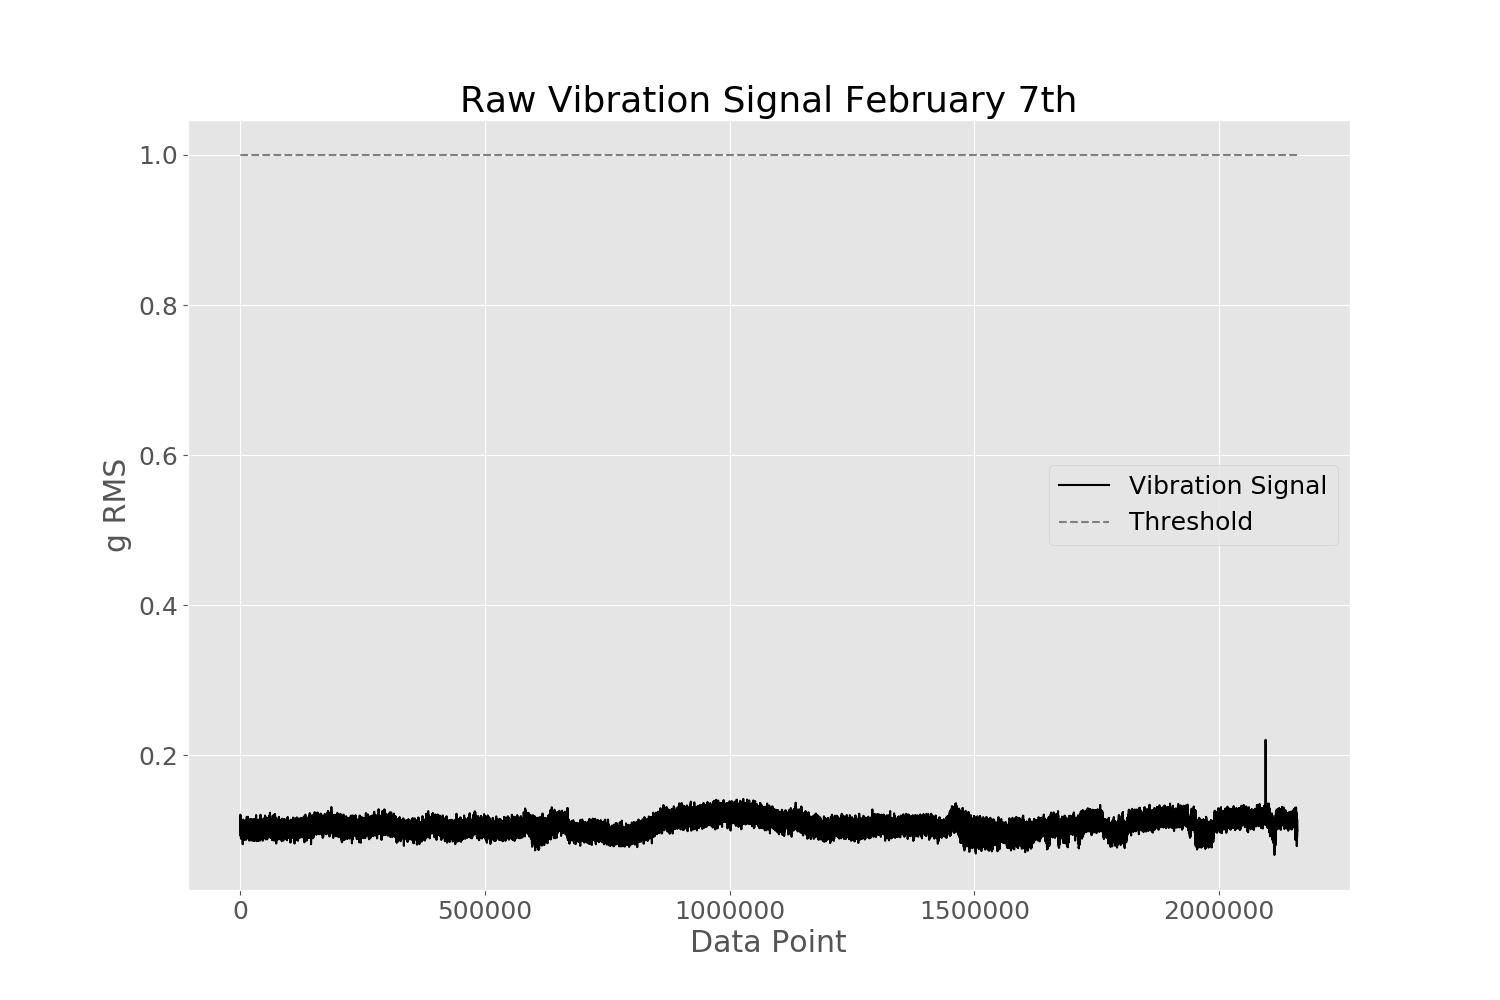
\includegraphics[trim={50 50 300 50}, width=\linewidth]{raw-feb7}
    \end{subfigure}
    \caption{Raw vibration signals.}
    \label{fig:raw-signals}
\end{figure}